\documentclass{article}

% Required packages
\usepackage{amssymb}
\usepackage{amsmath}
\usepackage{graphicx}
\usepackage{geometry}
\usepackage{tikz}
\usepackage{array}
\usepackage{booktabs}
\usepackage{enumitem}
\usepackage{listings}
\usepackage{xcolor}
\usepackage{fancyhdr}
\usepackage{longtable}
\usepackage{multirow}
\usepackage{float}
\usepackage{url}

% Set page geometry
\geometry{a4paper, margin=1in}

% Configure listings for Python
\lstset{
  language=Python,
  basicstyle=\ttfamily\footnotesize,
  numbers=left,
  numberstyle=\tiny\color{gray},
  frame=single,
  breaklines=true,
  breakatwhitespace=true,
  captionpos=b,
  tabsize=4,
  showspaces=false,
  showstringspaces=false,
  showtabs=false,
  commentstyle=\color{gray}\textit,
  keywordstyle=\color{blue}\bfseries,
  stringstyle=\color{red}
}

\begin{document}

\begin{center}
\Large\textbf{288R Project Progress Report - Physics-Informed Machine Learning for Regional Geomagnetic Hazard Forecasting}\\
\Large\textbf{Project Group \#: 6}\\
\Large\textbf{Authors: R.Scotty Rogers}\\
\Large\textbf{Emails: rsrogers@ucsd.edu}\\
\end{center}

\section*{1. Background}

Geomagnetic substorms, driven by solar wind-magnetosphere coupling, produce auroral electrojet intensifications that induce hazardous currents in ground-based infrastructure. The ability to forecast regional geomagnetic perturbations at specific high-latitude stations provides actionable lead time for power grid operators and pipeline engineers. This project develops a physics-informed machine learning pipeline that fuses multi-source geophysical data to predict station-level disturbances at Abisko (ABK), Bj\o rn\o ya (BJN), and Troms\o (TRO), replacing computationally expensive first-principles magnetosphere models with data-driven approximations that preserve physical interpretability.

\section*{2. Dataset Name and Citation/Link}

The analysis integrates five publicly available geophysical archives, selected to trace the complete Sun-to-ground causal chain:

\begin{table}[H]
\centering
\begin{tabular}{lllp{5cm}}
\toprule
\textbf{Layer} & \textbf{Source} & \textbf{Data Product} & \textbf{Citation/Access} \\
\midrule
Solar & GOES XRS & 0.05--0.8 nm X-ray irradiance, 1-min & NOAA NCEI, \url{https://data.ngdc.noaa.gov/platforms/solar-space-observing-satellites/goes/} \\
L1 & OMNI & Solar wind, IMF, plasma, 1-min merge & NASA/GSFC SPDF, \url{https://omniweb.gsfc.nasa.gov/form/sc_merge_min1.html} \\
GEO & GOES MAG & Magnetometer at 6.6 $R_E$, 1-min avg & NOAA NCEI, \url{https://data.ngdc.noaa.gov/platforms/solar-space-observing-satellites/goes/} \\
LEO & Swarm & Magnetic field at $\sim$500 km, 1 Hz & ESA, \url{https://swarm-diss.eo.esa.int/} \\
Ground & SuperMAG & Ground magnetometer 1-min & JHU APL, \url{https://supermag.jhuapl.edu/} \\
\bottomrule
\end{tabular}
\caption{Data sources organized by observation layer in the Sun-to-ground causal chain.}
\end{table}

\section*{3. Data Pipeline}

\subsection*{3.1 Purpose}

Fuse five geophysical data sources into a single temporally aligned feature matrix for supervised learning. Sources span the Sun-to-ground causal chain.

\subsection*{3.2 Pipeline Design and Details}

\textbf{Implementation:} Processing 118 monthly files (100 GB raw $\to$ 4.01 GB fused parquet).

\textbf{Merging:} Timestamp alignment at 1-minute resolution. Sources have different native cadences:
\begin{itemize}
  \item GOES XRS: 1-minute averaged X-ray flux
  \item OMNI: 1-minute merged solar wind (with gaps during satellite handovers)
  \item GOES MAG: 1-minute magnetometer averages
  \item Swarm: 1 Hz magnetic field (downsampled to 1-minute MLT-binned averages)
  \item SuperMAG: 1-minute ground magnetometer data
\end{itemize}

\textbf{Cleansing:} 
\begin{itemize}
  \item Flagged/saturation values mapped to NULL
  \item Physically impossible readings removed (e.g., negative X-ray flux)
  \item Station-specific missingness preserved as NULL (not imputed at this stage)
\end{itemize}

\textbf{Augmentation/Enrichment:}
\begin{itemize}
  \item \textbf{Lag features:} Encode propagation delays (XRS$\to$L1 $\sim$1hr, L1$\to$magnetopause $\sim$30min)
  \item \textbf{Rolling statistics:} 10/30/60-minute windows for sustained driving conditions
  \item \textbf{Cyclical encodings:} sin/cos for hour-of-day and day-of-year
  \item \textbf{Physics-derived:} Newell coupling function $\Phi = V^{4/3} |B_T \sin^3(\theta/2)|$
  \item \textbf{Missingness flags:} Binary indicators per source (gap becomes signal)
\end{itemize}

\textbf{Normalization:} Z-score standardization using training-set statistics only (2015--2023). Applied frozen to 2024 test data.

\section*{4. EDA Description}

EDA combined univariate, multivariate, graphical, and non-graphical methods
across four areas: data quality, distributions, outliers, and correlations.

\textbf{Distributions.} Kernel density estimation of $|dB/dt|$ across all
three stations (Figure~1) reveals extreme right skew and leptokurtosis
(ABK: skew=11.47, kurt=337.97; BJN: skew=7.94, kurt=138.58; TRO:
skew=9.46, kurt=212.26). The 0.3~nT/s event threshold falls deep in the
right tail, confirming severe class imbalance and motivating HSS, BSS, and
ROC-AUC as primary metrics over accuracy. Station curves differ in tail
weight, supporting separate station-specific models.

\textbf{Temporal structure.} Monthly event rates (Figure~2) cluster during
2015--2018 and 2023--2024, consistent with Solar Cycle 24 peak and Solar
Cycle 25 ascent, with a deep suppression near Solar Minimum (2019--2020).
All train/test splits are enforced chronologically to prevent temporal
leakage.

\textbf{Data quality and correlations.} Missingness analysis confirmed
structured gaps across GOES, OMNI, Swarm, and SuperMAG sources. Where
gaps coincide with instrument saturation, missingness is treated as
potentially informative signal rather than noise. Spearman correlations
and lagged cross-correlations between solar wind drivers ($B_z$, dynamic
pressure, $v_{sw}$) and $|dB/dt|$ guided feature selection and lag window
sizing. Full missingness heatmaps and correlation heatmaps are in
preparation.

\begin{figure}[H]
  \centering
  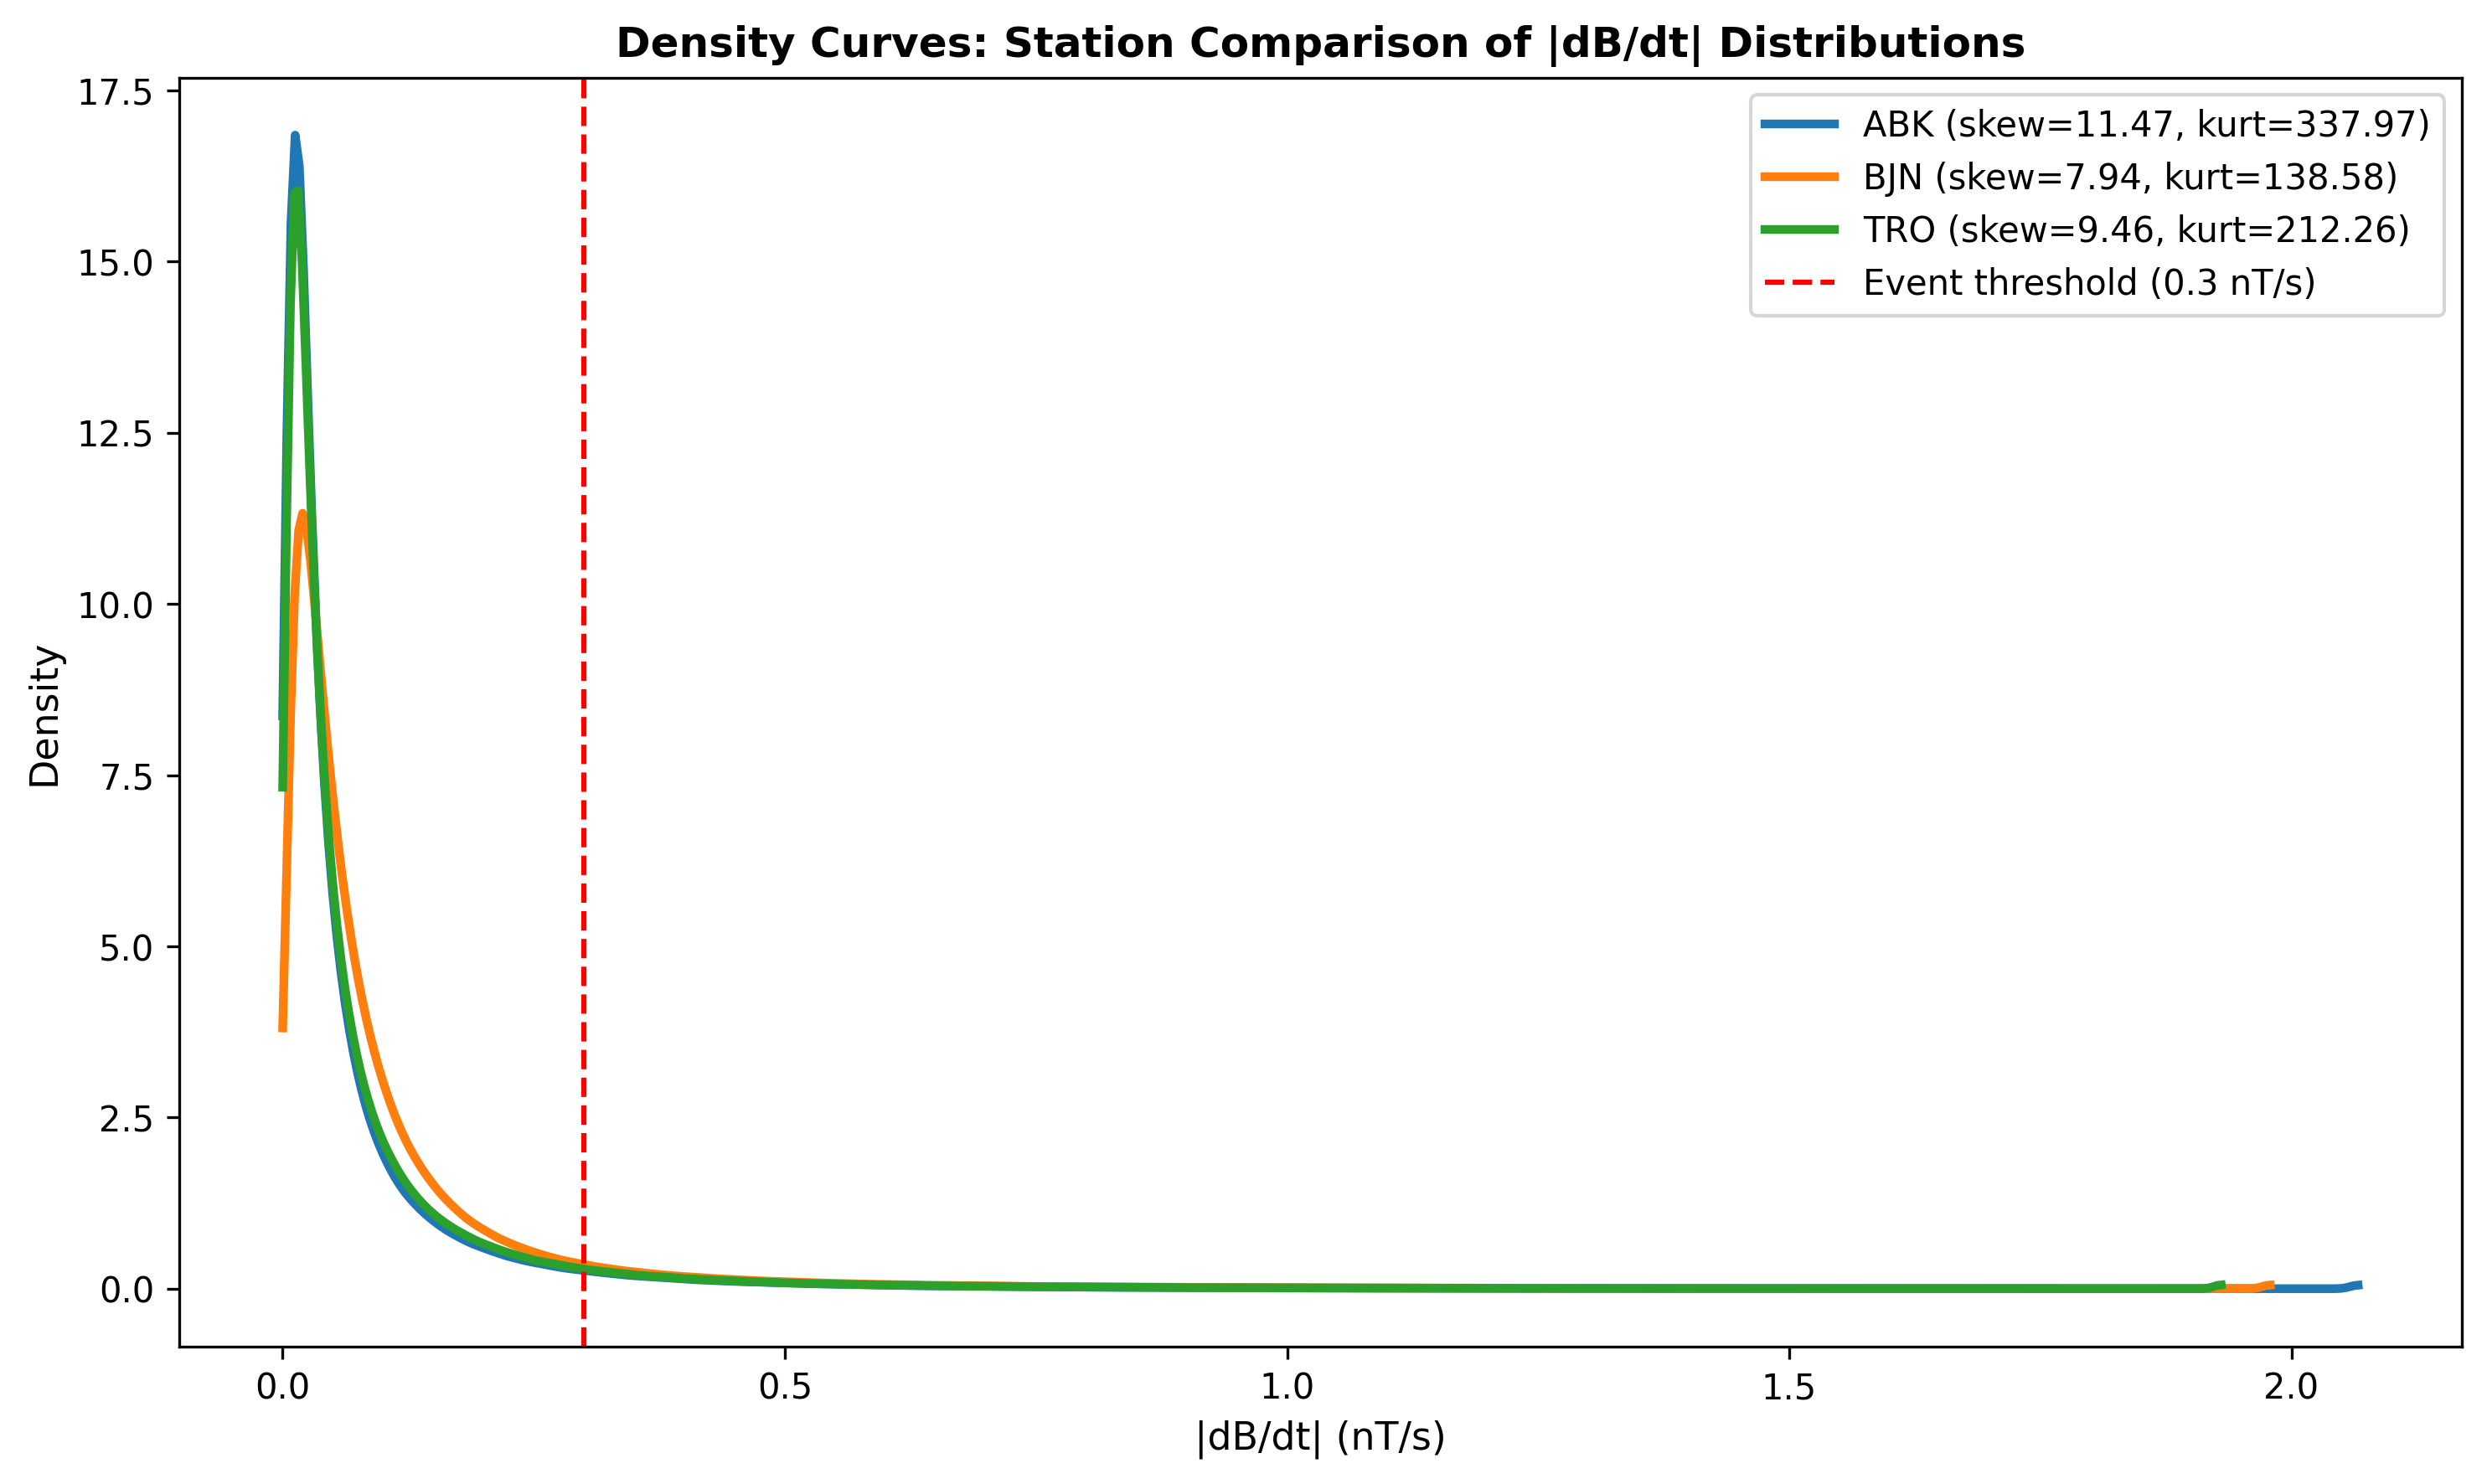
\includegraphics[width=0.85\textwidth]{eda_density_curves_stations.png}
  \caption{Kernel density estimates of $|dB/dt|$ for ABK, BJN, and TRO.
  The 0.3~nT/s event threshold (red dashed) sits in the extreme right
  tail, confirming rare-event class imbalance across all stations.}
\end{figure}

\begin{figure}[H]
  \centering
  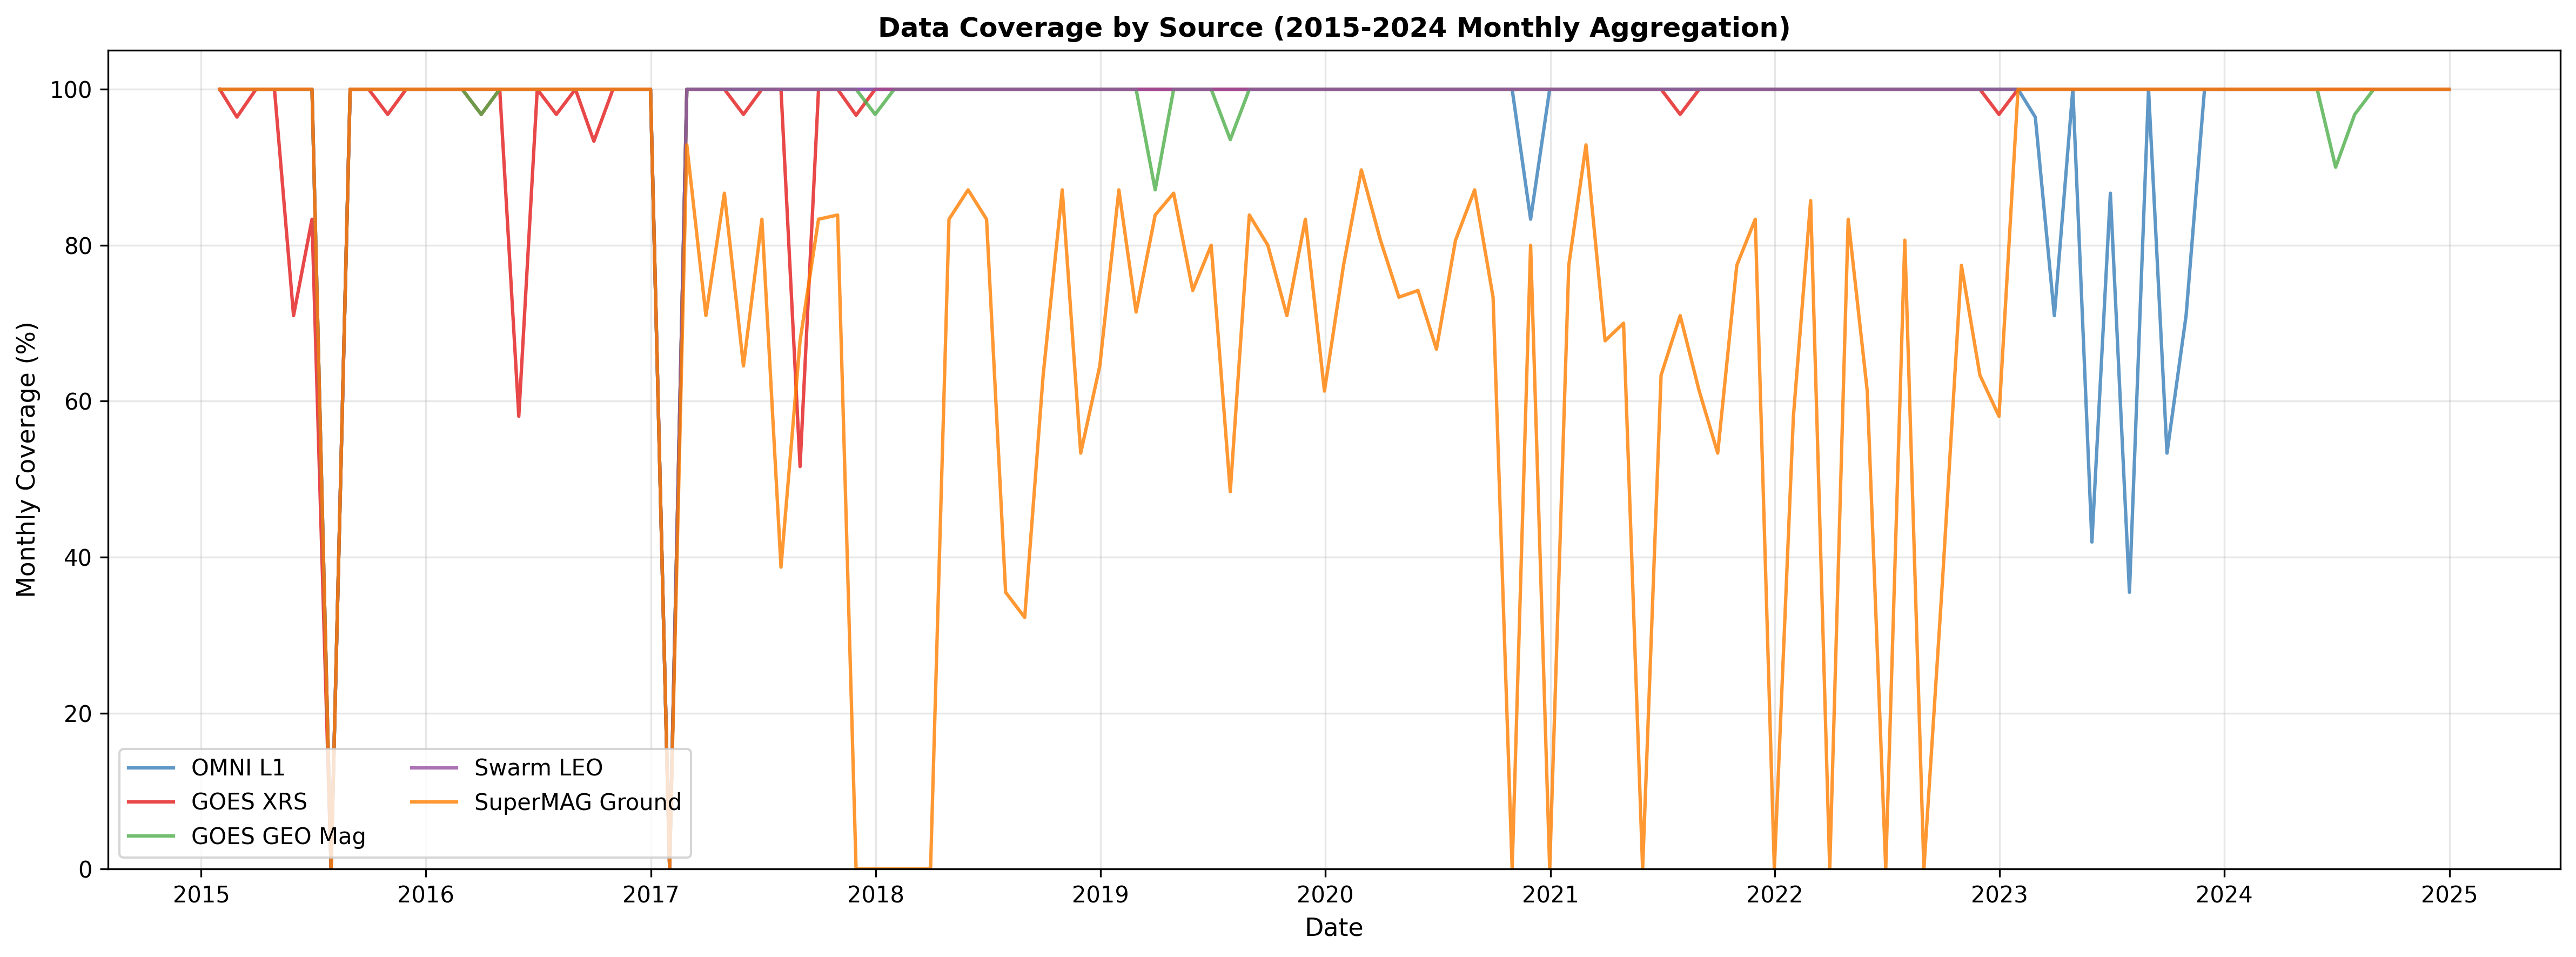
\includegraphics[width=0.85\textwidth]{eda_temporal_coverage.png}
  \caption{Monthly geomagnetic event rate per station (2015--2024).
  Activity clusters align with Solar Cycle 24 peak and Solar Cycle 25
  ascent, motivating chronological train/test splitting.}
\end{figure}

\section*{5. Feature Engineering}
Feature engineering (resulting in 129 total features across 14 categories) is explicitly traced to EDA findings:
\begin{itemize}[noitemsep]
    \item \textbf{EDA Trace 1 (Skewness):} Extreme right-skewed targets strictly dictate evaluating on thresholds like 0.3 nT/s rather than regression.
    \item \textbf{EDA Trace 2 (Correlations):} Strong correlations with \texttt{omni\_bz\_gsm} led to the inclusion of 10m/30m/60m rolling statistics to capture sustained physical drivers.
    \item \textbf{EDA Trace 3 (Gaps):} Missingness analysis revealed significant gaps (e.g., 24.1\% in ABK, 31.5\% in Newell $\Phi$). Gaps are treated as physical signals (missingness flags) rather than imputed noise.
    \item \textbf{EDA Trace 4 (Cyclicality):} UT/DOY seasonal patterns led to cyclical sine/cosine temporal encodings.
\end{itemize}

\section*{6. What Model(s) Are You Using? Justify}
Models are trained separately for each station (ABK, BJN, TRO) due to geographical and data missingness differences. 
\begin{itemize}[noitemsep]
    \item \textbf{Persistence \& Climatology:} Baseline sanity checks to establish minimal required skill (HSS).
    \item \textbf{Logistic Regression (Linear Benchmark):} Used strictly as a linear reference and probability calibration baseline. It tests whether complex non-linear interactions are necessary.
    \item \textbf{LightGBM (Primary Classifier):} Chosen natively to handle the extreme class imbalance, missingness-as-signal, and multiplicative physical interactions (like the Newell function).
    \item \textbf{LSTM (Planned):} A gray-box sequence model to explicitly test whether recurrent temporal memory provides skill beyond LightGBM's engineered rolling lags.
\end{itemize}

\section*{7. Progress Report}
The ETL and EDA pipelines are fully complete. 5.17 million rows of temporally aligned, multi-source data have been processed.
\begin{itemize}
    \item \textbf{Baselines executed:} Persistence sets a tough benchmark for this substorm tracking task. 
    \item \textbf{Model Execution:} Logistic Regression achieved high ROC-AUC (0.87--0.92) but severely poor calibration (BSS: -0.18 to -0.91, FAR $>$ 0.82). LightGBM similarly achieved good separation (ROC-AUC 0.81--0.88) but struggled with massive false alarm rates (FAR $>$ 0.91) due to extreme class imbalance. 
    \item \textbf{Feature Importance:} SHAP values confirm \texttt{goes\_bx/by}, \texttt{ut\_sin}, and \texttt{omni\_vx} are dominating the current LightGBM predictions.
\end{itemize}

\section*{8. Team Member Contribution (Solo)}
This is a solo project. All tasks completed by R. Scotty Rogers.
\begin{itemize}[noitemsep]
    \item \textbf{Completed:} Data fusion pipeline (118 files), automated EDA diagnostics, Feature Engineering (129 taxonomy traits), Baseline modeling (Persistence, Climatology, LR, LightGBM) with threshold tuning.
    \item \textbf{Planned:} Implement probability calibration, feature ablation studies, and LSTM architecture training.
\end{itemize}

\section*{9. Risks and Mitigation}
\begin{table}[H]
\centering
\begin{tabular}{p{4.5cm}p{10cm}}
\toprule
\textbf{Risk} & \textbf{Mitigation} \\
\midrule
Extreme Class Imbalance & Focus shifted from accuracy to threshold-tuned Heidke Skill Score (HSS) and ROC-AUC. \\
Poor Probability Calibration & Highly negative BSS scores across all ML models require immediate mitigation via Platt scaling or isotonic regression in Milestone 3. \\
Station Variability & Retaining separate, independent models for ABK, BJN, and TRO. \\
\bottomrule
\end{tabular}
\end{table}

\section*{10. References}

\begin{enumerate}
    \item Billcliff, N., et al. (2026). Extended lead-time geomagnetic storm forecasting with solar wind ensembles and machine learning. \textit{Space Weather}.
    \item Camporeale, E., et al. (2020). A gray-box model for a probabilistic estimate of regional ground magnetic perturbations. \textit{JGR: Space Physics}.
    \item Camporeale, E., et al. (2025). Verification of the NOAA SWPC solar flare forecast 1998--2024. \textit{Space Weather}.
    \item Chen, S., et al. (2025). GeoDGP: One-hour ahead global probabilistic geomagnetic perturbation forecasting. \textit{Space Weather}.
    \item Sun, Z., et al. (2022). A review of Earth artificial intelligence. \textit{Computers \& Geosciences}.
\end{enumerate}

\end{document}